\documentclass{article}
%--PASTE INTO MAIN FILE--
% \documentclass{article}
% %--PASTE INTO MAIN FILE--
% \documentclass{article}
% %--PASTE INTO MAIN FILE--
% \documentclass{article}
% \input{TexBase/DocumentBase.tex}
% \end{document}

\usepackage[margin = 0.7in]{geometry}
\usepackage{graphicx}
\usepackage{graphics}
\usepackage[T1]{fontenc}
\usepackage[polish]{babel}
\usepackage{cmap}
\usepackage[utf8]{inputenc}
\usepackage{float}
\usepackage{tabularx}
\usepackage[table,xcdraw]{xcolor}
\usepackage{lipsum}
\usepackage{titlesec}
\usepackage{minted}
\usepackage{xcolor}
\usepackage{caption}
\usepackage{enumitem}
\usepackage{csvsimple}
\usepackage{natbib}
\usepackage{blindtext}

\usepackage{amsmath} %math

\usepackage{numprint} % rounding
\usepackage[round-precision=3,round-mode=figures, scientific-notation=true]{siunitx} %scientific notation

\usepackage[hidelinks]{hyperref}
\usepackage{url}

\usepackage{bm} %bold for math


%TABS
\usepackage[]{booktabs}
\usepackage{tabularray}
\usepackage{multirow}

%\title{}
\author{Michał Dziedziak}
\date{\today}


\titlespacing\section{0pt}{12pt plus 4pt minus 2pt}{0pt plus 2pt minus 2pt}
\titlespacing\subsection{0pt}{12pt plus 4pt minus 2pt}{0pt plus 2pt minus 2pt}
\titlespacing\subsubsection{0pt}{12pt plus 4pt minus 2pt}{0pt plus 2pt minus 2pt}
\setlength{\parskip}{\baselineskip}%
\setlength{\parindent}{0pt}%

\newcommand{\squeezeup}{\vspace{-5mm}}


\begin{document}

\begin{titlepage}
    \begin{center}
        \vspace*{5cm}
        \rule{500pt}{1pt}\\
        \vspace*{0.5cm}
        \LARGE
        \textbf{Inżyniera Obrazów}\\
        \Large
        Laboratorium numer 2
        \vspace*{0.5cm}
        \rule{500pt}{1pt}
    \end{center}

    \vspace*{10cm}

    {\raggedright
        \large
        \textbf{Autor sprawozdania:} Michał Dziedziak 263901\\
        \textbf{Imię i Nazwisko prowadzącego kurs:} dr inż. Jan Nikodem\\
        \textbf{Dzień i godzina zajęć:} czwartek, 11:15 - 14:15
    }
\end{titlepage}


\tableofcontents
% \listoftables

%\renewcommand\listoflistingscaption{List of source codes}
% \listoflistings

\listoffigures


\newpage


% \begin{table}[H]
%     \centering
%     \begin{tabular}{|c|c|c|c|}%
%         \hline
%         \bfseries Numer iteracji & \bfseries Czas zalezienia rozwiązania [ms] & Koszt ścieżki & Błąd względny% specify table head
%         \csvreader[head to column names]{Csv/BestPathTest_SimulatedAnnealing_LINEAR_ftv47.csv}{}% use head of csv as column names
%         {\\\hline\Iteration & \num{\TimeInMiliSeconds} & \Cost & \num[round-precision=2, round-mode=places, scientific-notation=false]{\Error}\%}% specify your columns here
%         \\\hline    
%     \end{tabular}
%     \caption{}
%     \label{tab:}
% \end{table}

% \begin{figure}[H]
%     \centering
%     \resizebox{\columnwidth}{!}{%
%     \includegraphics{}%
%     }
%     \caption{}
%     \label{fig:}
% \end{figure}

% \begin{listing}[H]
%     \begin{minted}[frame=single,framesep=2mm,linenos,fontsize=\footnotesize]{language}
%         some code
%     \end{minted}
%     \caption{}
%     \label{lst:}
% \end{listing}


% \bibliographystyle{plainnat}
% \bibliography{TexBase/Bibliography}

% \end{document}

\usepackage[margin = 0.7in]{geometry}
\usepackage{graphicx}
\usepackage{graphics}
\usepackage[T1]{fontenc}
\usepackage[polish]{babel}
\usepackage{cmap}
\usepackage[utf8]{inputenc}
\usepackage{float}
\usepackage{tabularx}
\usepackage[table,xcdraw]{xcolor}
\usepackage{lipsum}
\usepackage{titlesec}
\usepackage{minted}
\usepackage{xcolor}
\usepackage{caption}
\usepackage{enumitem}
\usepackage{csvsimple}
\usepackage{natbib}
\usepackage{blindtext}

\usepackage{amsmath} %math

\usepackage{numprint} % rounding
\usepackage[round-precision=3,round-mode=figures, scientific-notation=true]{siunitx} %scientific notation

\usepackage[hidelinks]{hyperref}
\usepackage{url}

\usepackage{bm} %bold for math


%TABS
\usepackage[]{booktabs}
\usepackage{tabularray}
\usepackage{multirow}

%\title{}
\author{Michał Dziedziak}
\date{\today}


\titlespacing\section{0pt}{12pt plus 4pt minus 2pt}{0pt plus 2pt minus 2pt}
\titlespacing\subsection{0pt}{12pt plus 4pt minus 2pt}{0pt plus 2pt minus 2pt}
\titlespacing\subsubsection{0pt}{12pt plus 4pt minus 2pt}{0pt plus 2pt minus 2pt}
\setlength{\parskip}{\baselineskip}%
\setlength{\parindent}{0pt}%

\newcommand{\squeezeup}{\vspace{-5mm}}


\begin{document}

\begin{titlepage}
    \begin{center}
        \vspace*{5cm}
        \rule{500pt}{1pt}\\
        \vspace*{0.5cm}
        \LARGE
        \textbf{Inżyniera Obrazów}\\
        \Large
        Laboratorium numer 2
        \vspace*{0.5cm}
        \rule{500pt}{1pt}
    \end{center}

    \vspace*{10cm}

    {\raggedright
        \large
        \textbf{Autor sprawozdania:} Michał Dziedziak 263901\\
        \textbf{Imię i Nazwisko prowadzącego kurs:} dr inż. Jan Nikodem\\
        \textbf{Dzień i godzina zajęć:} czwartek, 11:15 - 14:15
    }
\end{titlepage}


\tableofcontents
% \listoftables

%\renewcommand\listoflistingscaption{List of source codes}
% \listoflistings

\listoffigures


\newpage


% \begin{table}[H]
%     \centering
%     \begin{tabular}{|c|c|c|c|}%
%         \hline
%         \bfseries Numer iteracji & \bfseries Czas zalezienia rozwiązania [ms] & Koszt ścieżki & Błąd względny% specify table head
%         \csvreader[head to column names]{Csv/BestPathTest_SimulatedAnnealing_LINEAR_ftv47.csv}{}% use head of csv as column names
%         {\\\hline\Iteration & \num{\TimeInMiliSeconds} & \Cost & \num[round-precision=2, round-mode=places, scientific-notation=false]{\Error}\%}% specify your columns here
%         \\\hline    
%     \end{tabular}
%     \caption{}
%     \label{tab:}
% \end{table}

% \begin{figure}[H]
%     \centering
%     \resizebox{\columnwidth}{!}{%
%     \includegraphics{}%
%     }
%     \caption{}
%     \label{fig:}
% \end{figure}

% \begin{listing}[H]
%     \begin{minted}[frame=single,framesep=2mm,linenos,fontsize=\footnotesize]{language}
%         some code
%     \end{minted}
%     \caption{}
%     \label{lst:}
% \end{listing}


% \bibliographystyle{plainnat}
% \bibliography{TexBase/Bibliography}

% \end{document}

\usepackage[margin = 0.7in]{geometry}
\usepackage{graphicx}
\usepackage{graphics}
\usepackage[T1]{fontenc}
\usepackage[polish]{babel}
\usepackage{cmap}
\usepackage[utf8]{inputenc}
\usepackage{float}
\usepackage{tabularx}
\usepackage[table,xcdraw]{xcolor}
\usepackage{lipsum}
\usepackage{titlesec}
\usepackage{minted}
\usepackage{xcolor}
\usepackage{caption}
\usepackage{enumitem}
\usepackage{csvsimple}
\usepackage{natbib}
\usepackage{blindtext}

\usepackage{amsmath} %math

\usepackage{numprint} % rounding
\usepackage[round-precision=3,round-mode=figures, scientific-notation=true]{siunitx} %scientific notation

\usepackage[hidelinks]{hyperref}
\usepackage{url}

\usepackage{bm} %bold for math


%TABS
\usepackage[]{booktabs}
\usepackage{tabularray}
\usepackage{multirow}

%\title{}
\author{Michał Dziedziak}
\date{\today}


\titlespacing\section{0pt}{12pt plus 4pt minus 2pt}{0pt plus 2pt minus 2pt}
\titlespacing\subsection{0pt}{12pt plus 4pt minus 2pt}{0pt plus 2pt minus 2pt}
\titlespacing\subsubsection{0pt}{12pt plus 4pt minus 2pt}{0pt plus 2pt minus 2pt}
\setlength{\parskip}{\baselineskip}%
\setlength{\parindent}{0pt}%

\newcommand{\squeezeup}{\vspace{-5mm}}


\begin{document}

\begin{titlepage}
    \begin{center}
        \vspace*{5cm}
        \rule{500pt}{1pt}\\
        \vspace*{0.5cm}
        \LARGE
        \textbf{Inżyniera Obrazów}\\
        \Large
        Laboratorium numer 2
        \vspace*{0.5cm}
        \rule{500pt}{1pt}
    \end{center}

    \vspace*{10cm}

    {\raggedright
        \large
        \textbf{Autor sprawozdania:} Michał Dziedziak 263901\\
        \textbf{Imię i Nazwisko prowadzącego kurs:} dr inż. Jan Nikodem\\
        \textbf{Dzień i godzina zajęć:} czwartek, 11:15 - 14:15
    }
\end{titlepage}


\tableofcontents
% \listoftables

%\renewcommand\listoflistingscaption{List of source codes}
% \listoflistings

\listoffigures


\newpage


% \begin{table}[H]
%     \centering
%     \begin{tabular}{|c|c|c|c|}%
%         \hline
%         \bfseries Numer iteracji & \bfseries Czas zalezienia rozwiązania [ms] & Koszt ścieżki & Błąd względny% specify table head
%         \csvreader[head to column names]{Csv/BestPathTest_SimulatedAnnealing_LINEAR_ftv47.csv}{}% use head of csv as column names
%         {\\\hline\Iteration & \num{\TimeInMiliSeconds} & \Cost & \num[round-precision=2, round-mode=places, scientific-notation=false]{\Error}\%}% specify your columns here
%         \\\hline    
%     \end{tabular}
%     \caption{}
%     \label{tab:}
% \end{table}

% \begin{figure}[H]
%     \centering
%     \resizebox{\columnwidth}{!}{%
%     \includegraphics{}%
%     }
%     \caption{}
%     \label{fig:}
% \end{figure}

% \begin{listing}[H]
%     \begin{minted}[frame=single,framesep=2mm,linenos,fontsize=\footnotesize]{language}
%         some code
%     \end{minted}
%     \caption{}
%     \label{lst:}
% \end{listing}


% \bibliographystyle{plainnat}
% \bibliography{TexBase/Bibliography}



\section{Temat laboratorium}
W ramach piątych zajęć laboratoryjnych:
\begin{itemize}
    \item Poznaliśmy czym jest ditering, oraz jakie są jego zastosowania.
    \item Poznaliśmy algorytmy do rysowania lini i trójkątów w obrazie.
    \item Poznaliśmy czym jest SSAA
\end{itemize}

\section{Zadanie 1}

\subsection{Zadania do wykonania}
Zadanie pierwsze polegało na zaimplementowaniu ditheringu dla obrazu w skali szarości. W tym celu wykonałem
następujące kroki:
\begin{enumerate}
    \item Przeniosłem obraz z przestrzeni barw RGB na skalę szarości.
    \item Użyłem algorytmu Floyda-Steinberga do nałożenia ditheringu na obraz.
    \item Wyświetliłem obraz oryginalny, obraz po redukcji kolorów i obraz przetworzony.
\end{enumerate}

\subsection{Teoria}

\subsubsection*{Redukcja palety barw}
Redukcja palety kolorów obrazu polega na zmniejszeniu liczby unikalnych kolorów w celu uproszczenia danych
obrazu, zmniejszenia zużycia pamięci lub uzyskania określonego efektu wizualnego. Typowo każdą składową koloru
reprezentujemy jako jedną z 256 wartości, co daje 16 777 216 unikalnych odcieni. Niektóre urządzenia i formaty
graficzne są ograniczone w tej kwestii, co skutkuje mniejszą liczbą dostępnych odcieni.

Redukcja palety kolorów zmniejsza liczbę tych odcieni, mapując każdą wartość koloru do najbliższego
odpowiednika w ograniczonej przestrzeni kolorów. Na przykład, przy redukcji do dwóch kolorów (czarny i biały),
wartości kolorów poniżej 128 są zaokrąglane do 0 (czarny), a powyżej 128 do 255 (biały).

W obrazach RGB zmniejsza się paletę kolorów dla każdego z kanałów osobno, traktując każdy kanał jako oddzielny
obraz w skali szarości. Rezultatem jest obraz używający mniej unikalnych kolorów, ale zachowujący ogólną strukturę i wygląd oryginału.

Źródła: \cite{DitheringDlaObrazówKolorowych1}, \cite{DitheringDlaObrazówKolorowych2}

\subsubsection*{Dithering}
Dithering to technika stosowana w grafice komputerowej w celu symulacji większej liczby kolorów i odcieni w
obrazach o ograniczonej palecie kolorów. Polega na rozmieszczaniu pikseli o różnych kolorach w taki sposób, aby stworzyć
iluzję dodatkowych kolorów i płynniejszych przejść tonalnych.

Dithering działa poprzez wprowadzanie drobnych, losowych wzorców lub regularnych układów pikseli, które
ludzkie oko interpretuje jako nowe odcienie. Na przykład, na obrazie zredukowanym do czerni i bieli, dithering może
mieszać czarne i białe piksele, aby zasymulować odcienie szarości.

Źródła: \cite{DitheringDlaObrazówKolorowych2}, \cite{Dithering}


\subsubsection*{Algorytm Floyda-Steinberga}
Algorytm Floyda-Steinberga to jeden z najpopularniejszych algorytmów ditheringu, stosowany do poprawy jakości
obrazów o ograniczonej liczbie kolorów. Algorytm ten jest techniką ditheringu rozproszonego błędu (error
diffusion dithering),
co oznacza, że błąd powstały podczas kwantyzacji koloru jest rozpraszany na sąsiednie piksele, co skutkuje
bardziej naturalnym wyglądem obrazu.

Algorytm Floyda-Steinberga działa w następujący sposób:
\begin{enumerate}
    \item Kwantyzacja piksela: Każdy piksel w obrazie jest przetwarzany pojedynczo. Kolor aktualnego piksela jest
          zaokrąglany do najbliższego koloru w ograniczonej palecie.
    \item Obliczenie błędu: Błąd kwantyzacji jest różnicą między oryginalnym kolorem piksela a nowym kolorem po
          kwantyzacji.
    \item Rozproszenie błędu: Błąd ten jest następnie rozpraszany na sąsiednie piksele, które jeszcze nie zostały
          przetworzone. Rozproszenie błędu odbywa się według macierzy:
          \[
              \begin{bmatrix}
                  -    & *    & 7/17 \\
                  3/16 & 5/16 & 1/16
              \end{bmatrix}
          \]
          Dodajemy błąd przeskalowany przez wartość z macierzy do pikseli sąsiednich (względem piksela oznaczonego \*).
\end{enumerate}

Źródła: \cite{DitheringDlaObrazówKolorowych2}, \cite{Dithering}

\subsection{Prezentacja wykonanego zadania}
\begin{figure}[H]
    \centering
    \resizebox{\columnwidth}{!}{%
        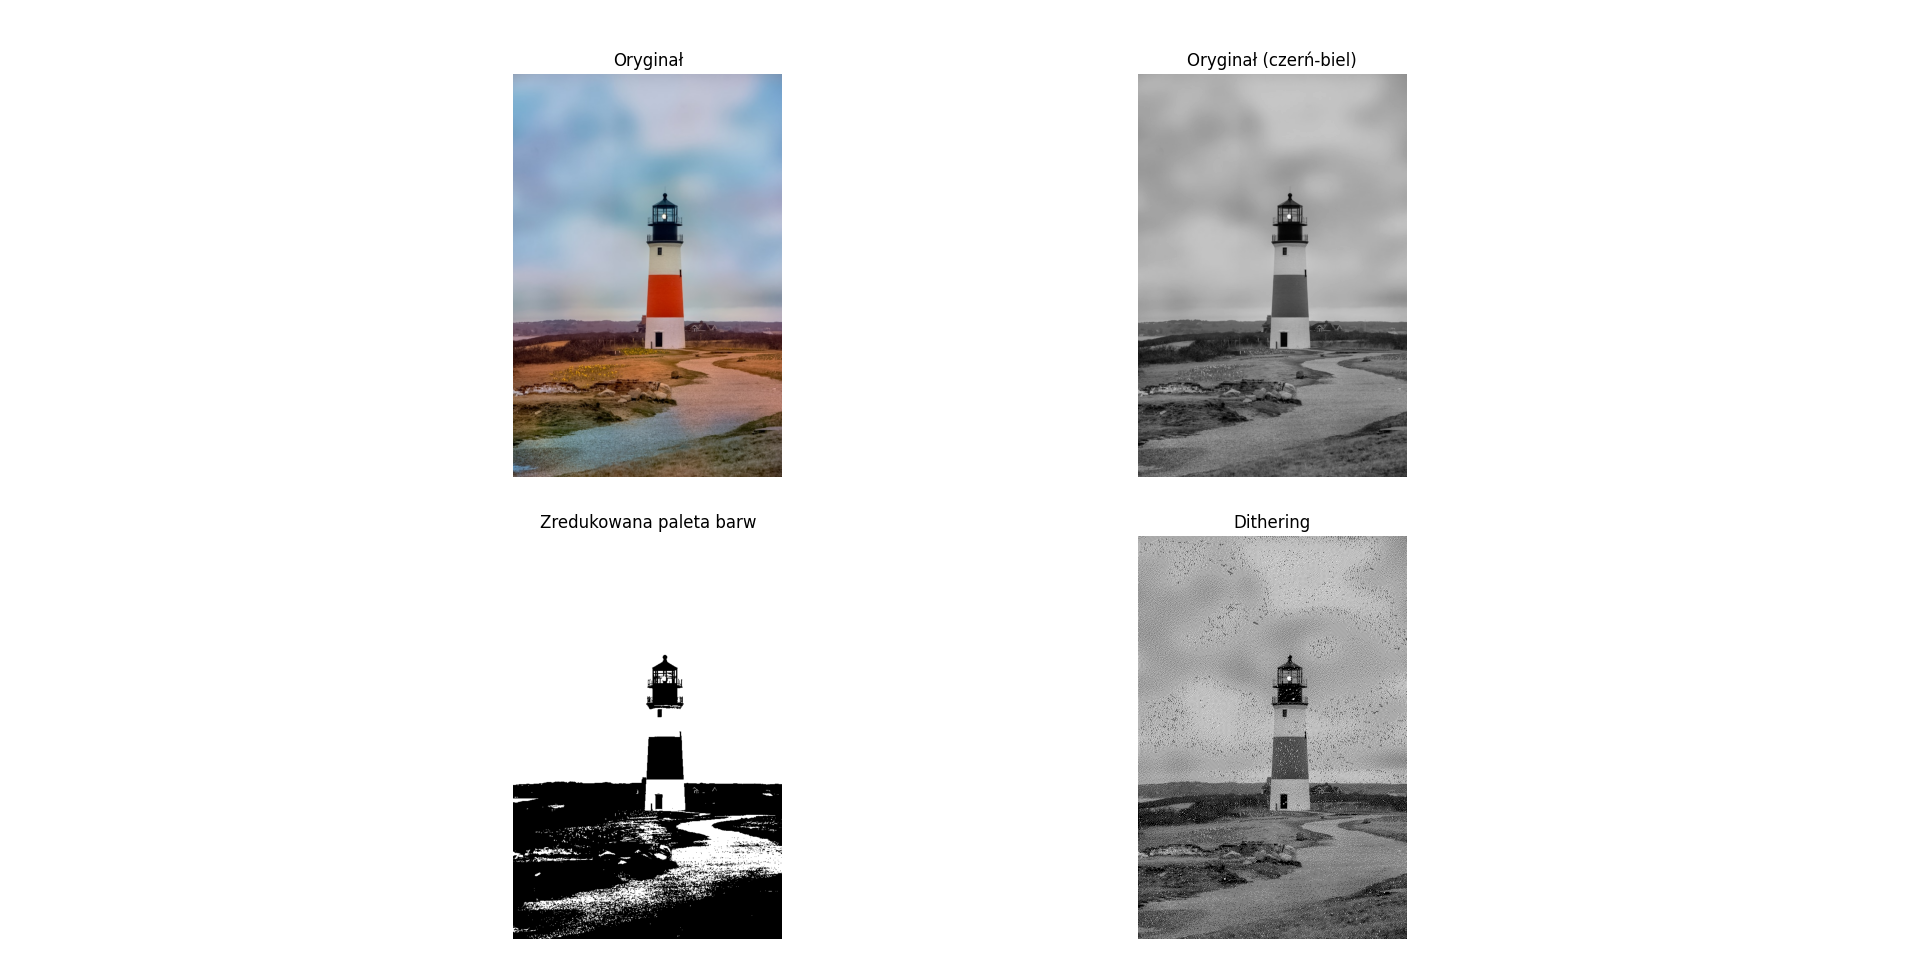
\includegraphics{Img/zad1.png}%
    }
    \caption{Zdjęcie przedstawiające obraz oryginalny, obraz w skali szarości, obraz po redukcji kolorów i obraz po przetworzeniu.}
\end{figure}

\begin{figure}[H]
    \centering
    \resizebox{\columnwidth}{!}{%
        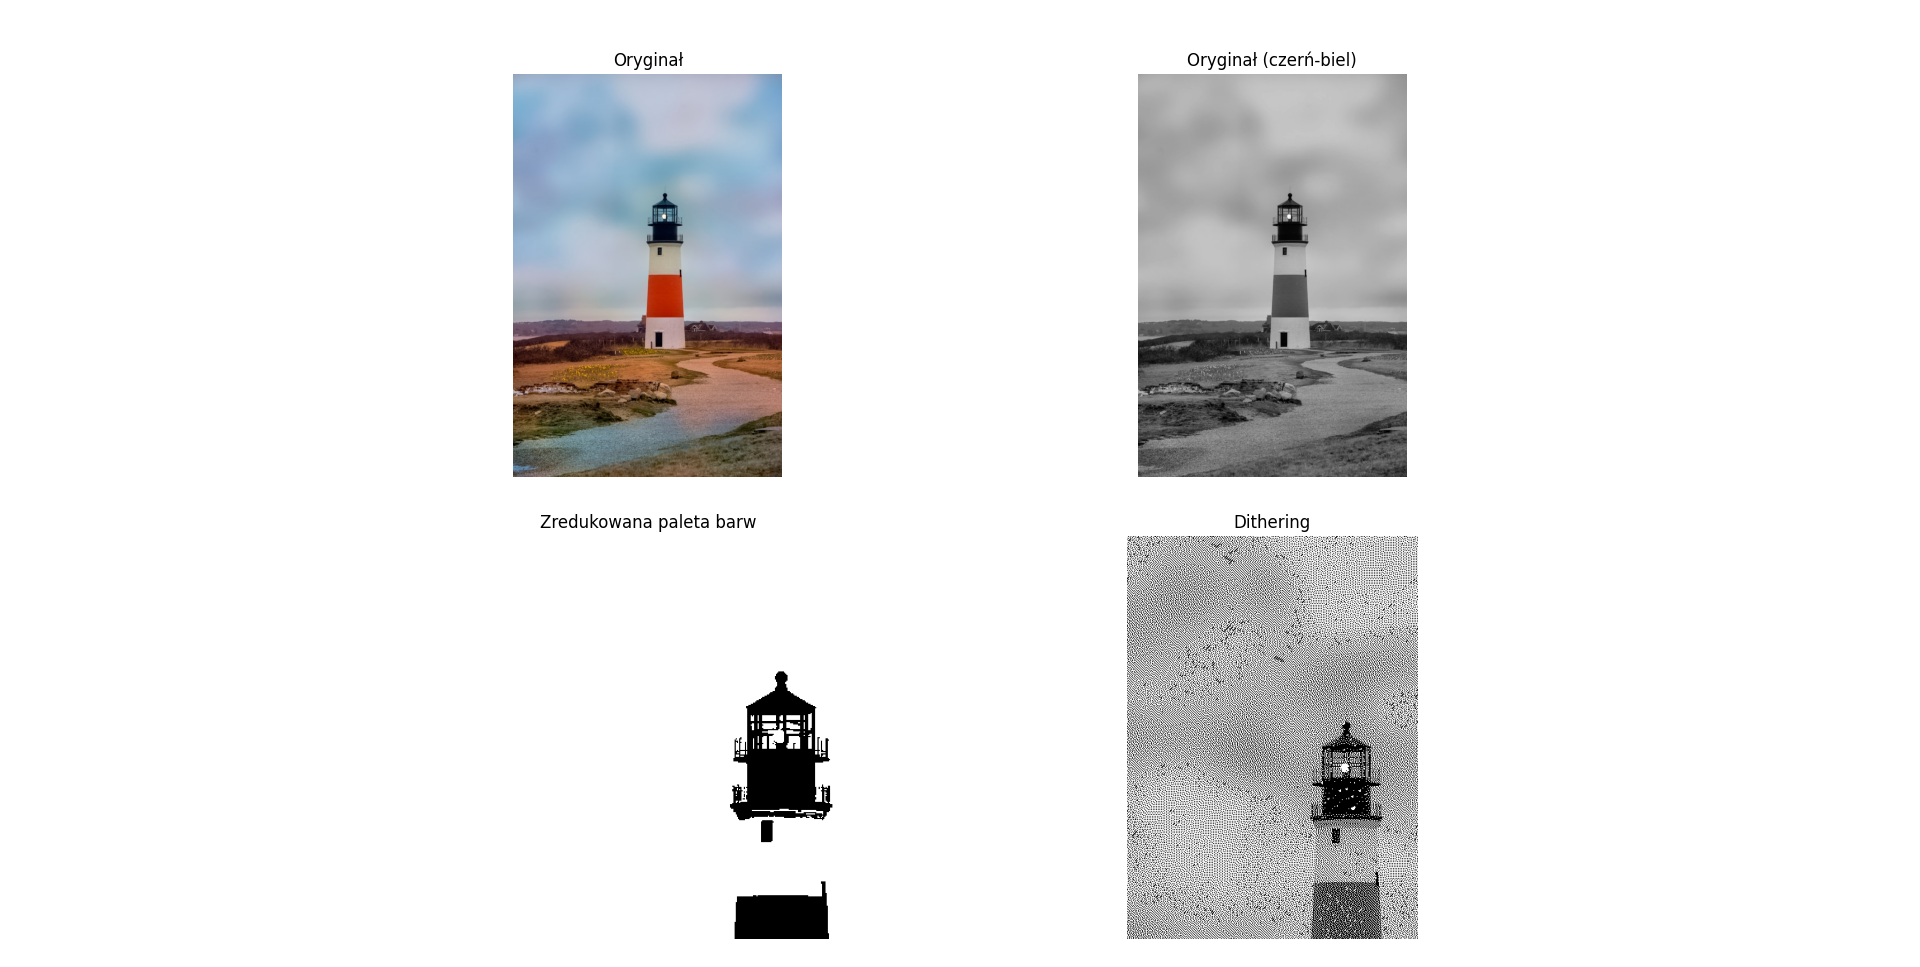
\includegraphics{Img/zad1_2.png}%
    }
    \caption{Zdjęcie przedstawiające obraz oryginalny, obraz w skali szarości, przybliżony obraz po redukcji kolorów i przybliżony obraz po przetworzeniu.}
\end{figure}


\section{Zadanie 2}

\subsection{Zadania do wykonania}
Zadanie drugie polegało na zaimplementowaniu ditheringu dla obrazu w kolorze.
Wykonane kroki były analogiczne do poprzedniego zadania, z tą różnicą, że kazdy kanał koloru był przetwarzany osobno.

Dodatkowo została zaimplementowana możliwość wyboru liczby kolorów, do których ma zostać zredukowana paleta.

\subsection{Prezentacja wykonanego zadania}
\begin{figure}[H]
    \centering
    \resizebox{\columnwidth}{!}{%
        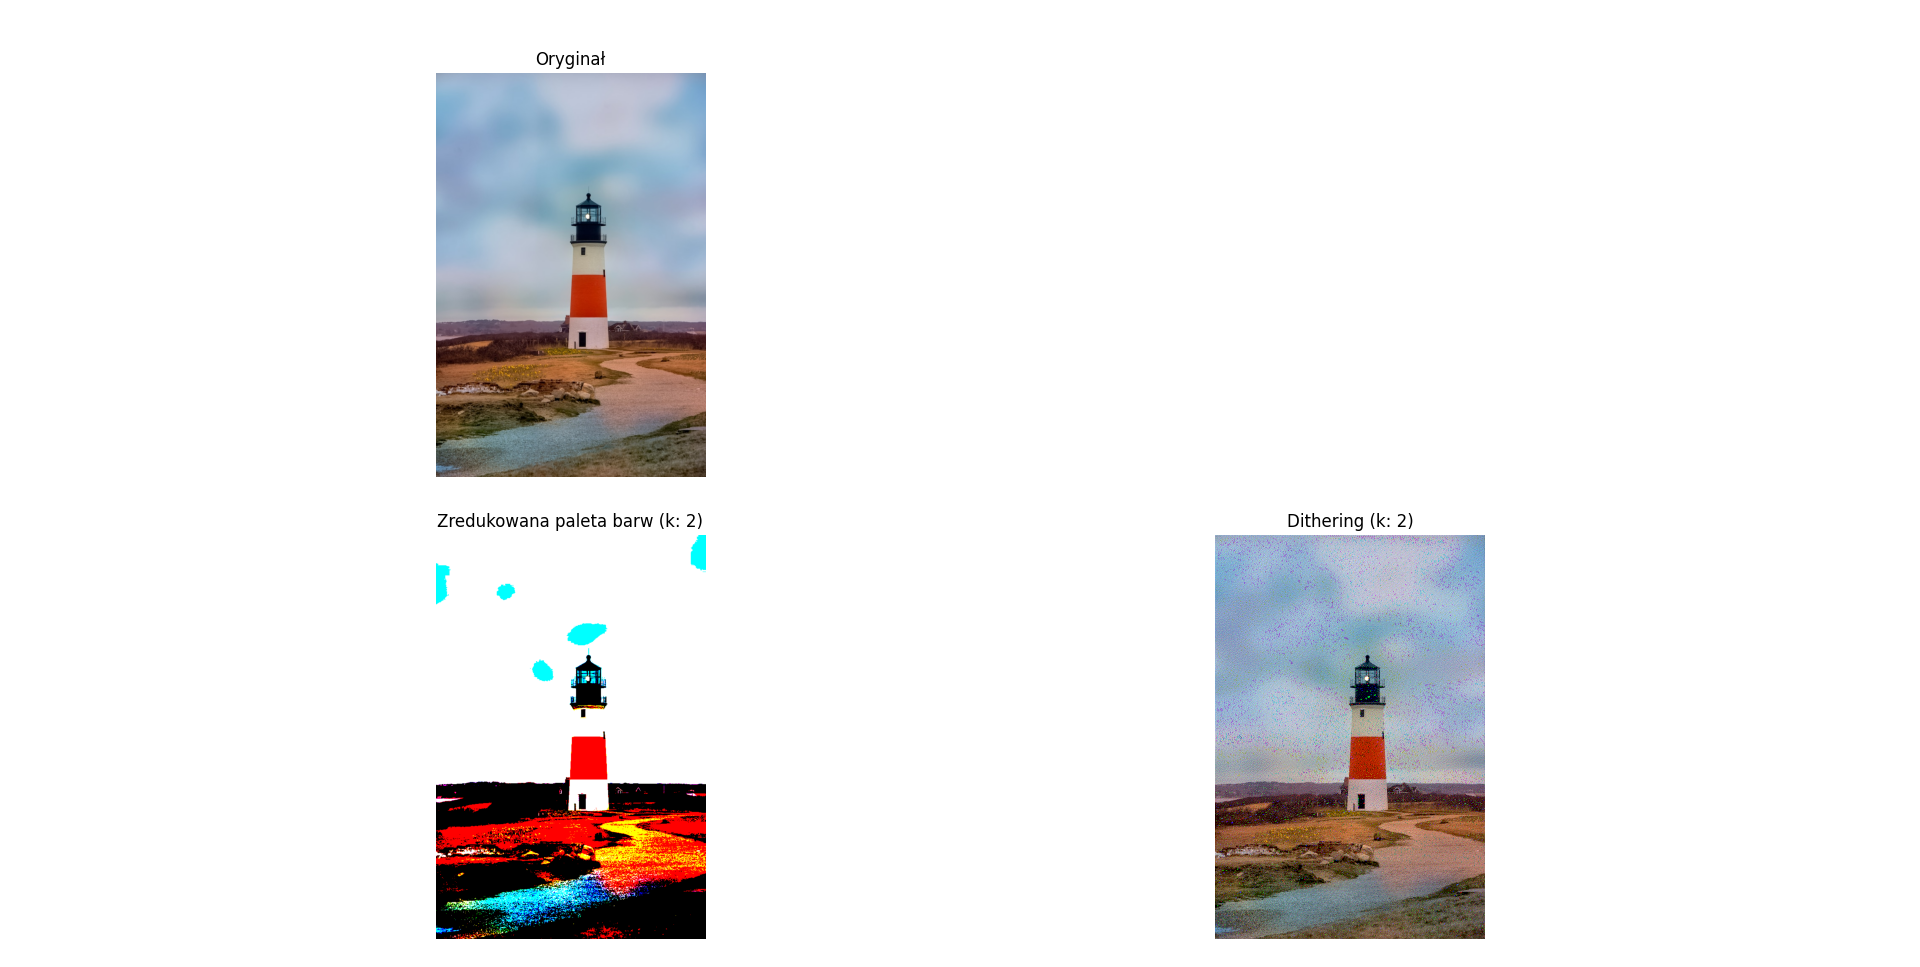
\includegraphics{Img/zad2.png}%
    }
    \caption{Zdjęcie przedstawiające obraz oryginalny, obraz po redukcji kolorów i obraz po przetworzeniu (dla k = 2).}
\end{figure}

\begin{figure}[H]
    \centering
    \resizebox{\columnwidth}{!}{%
        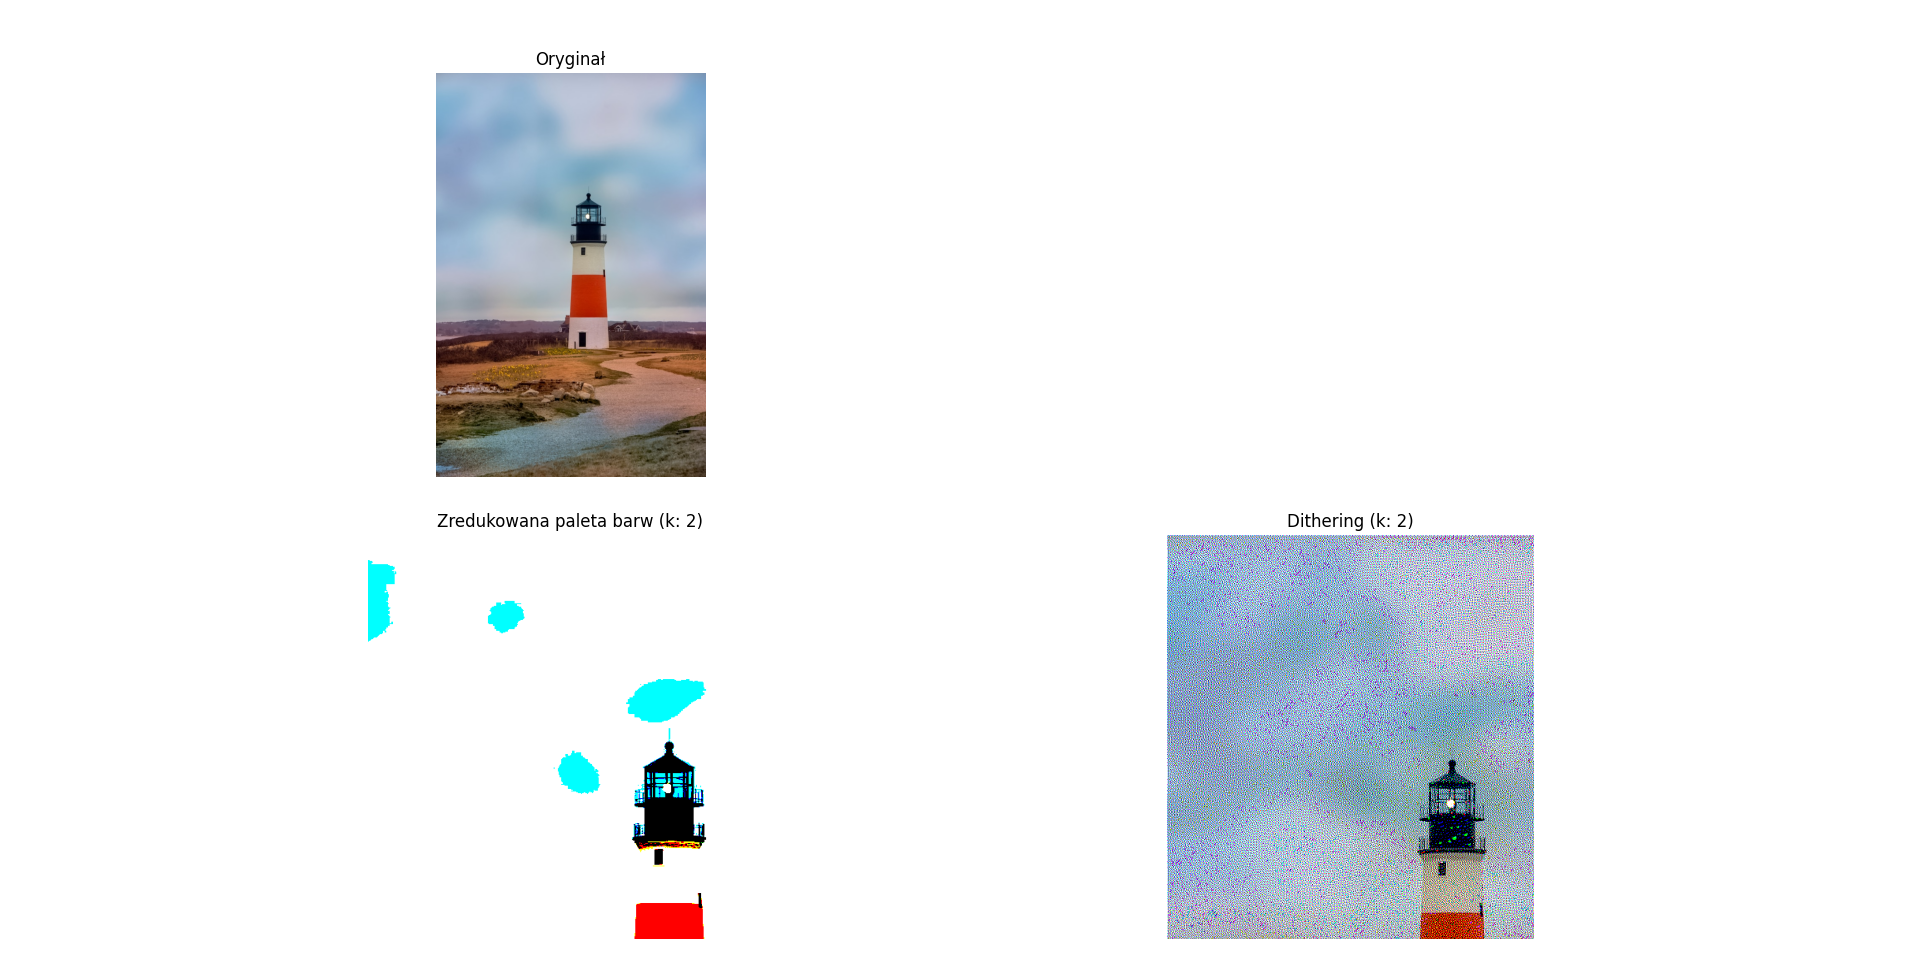
\includegraphics{Img/zad2_2.png}%
    }
    \caption{Zdjęcie przedstawiające obraz oryginalny, przybliżony obraz po redukcji kolorów i przybliżony obraz po przetworzeniu (dla k = 2).}
\end{figure}

\begin{figure}[H]
    \centering
    \resizebox{\columnwidth}{!}{%
        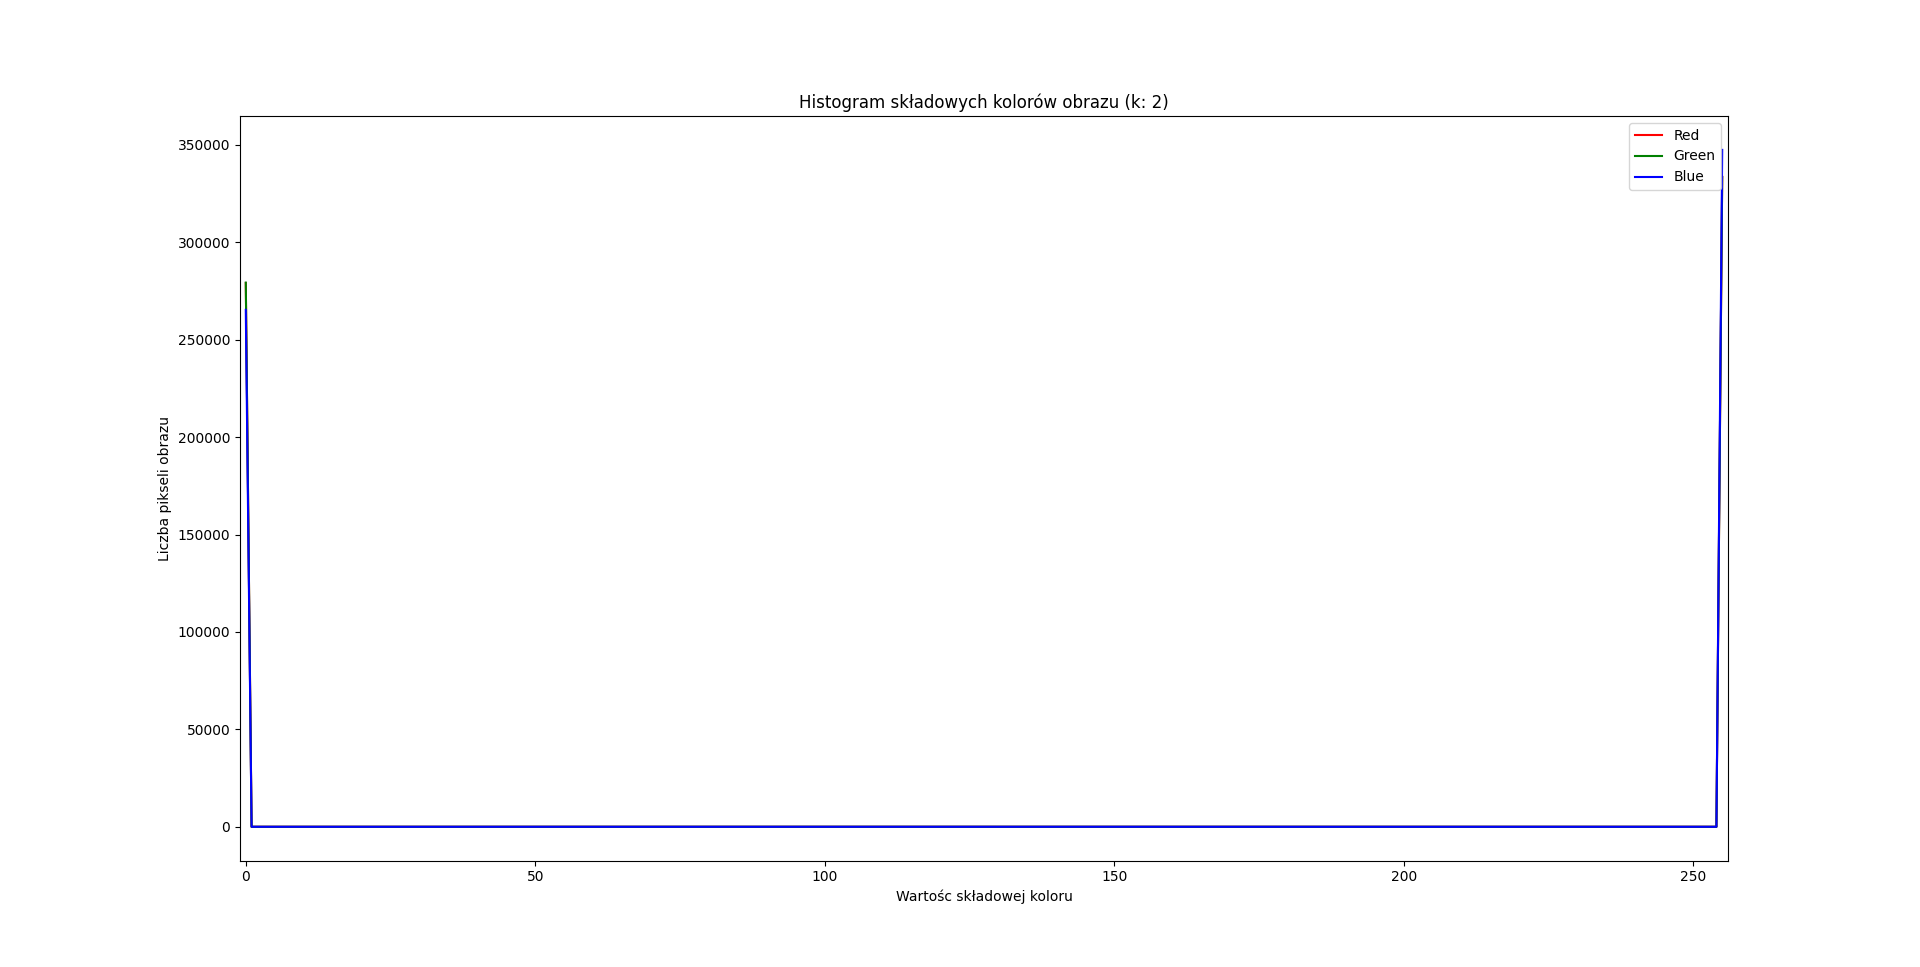
\includegraphics{Img/zad2_3.png}%
    }
    \caption{Zdjęcie przedstawiające histogram składowych kolorów przetworzonego obrazu dla k = 2}
\end{figure}

\begin{figure}[H]
    \centering
    \resizebox{\columnwidth}{!}{%
        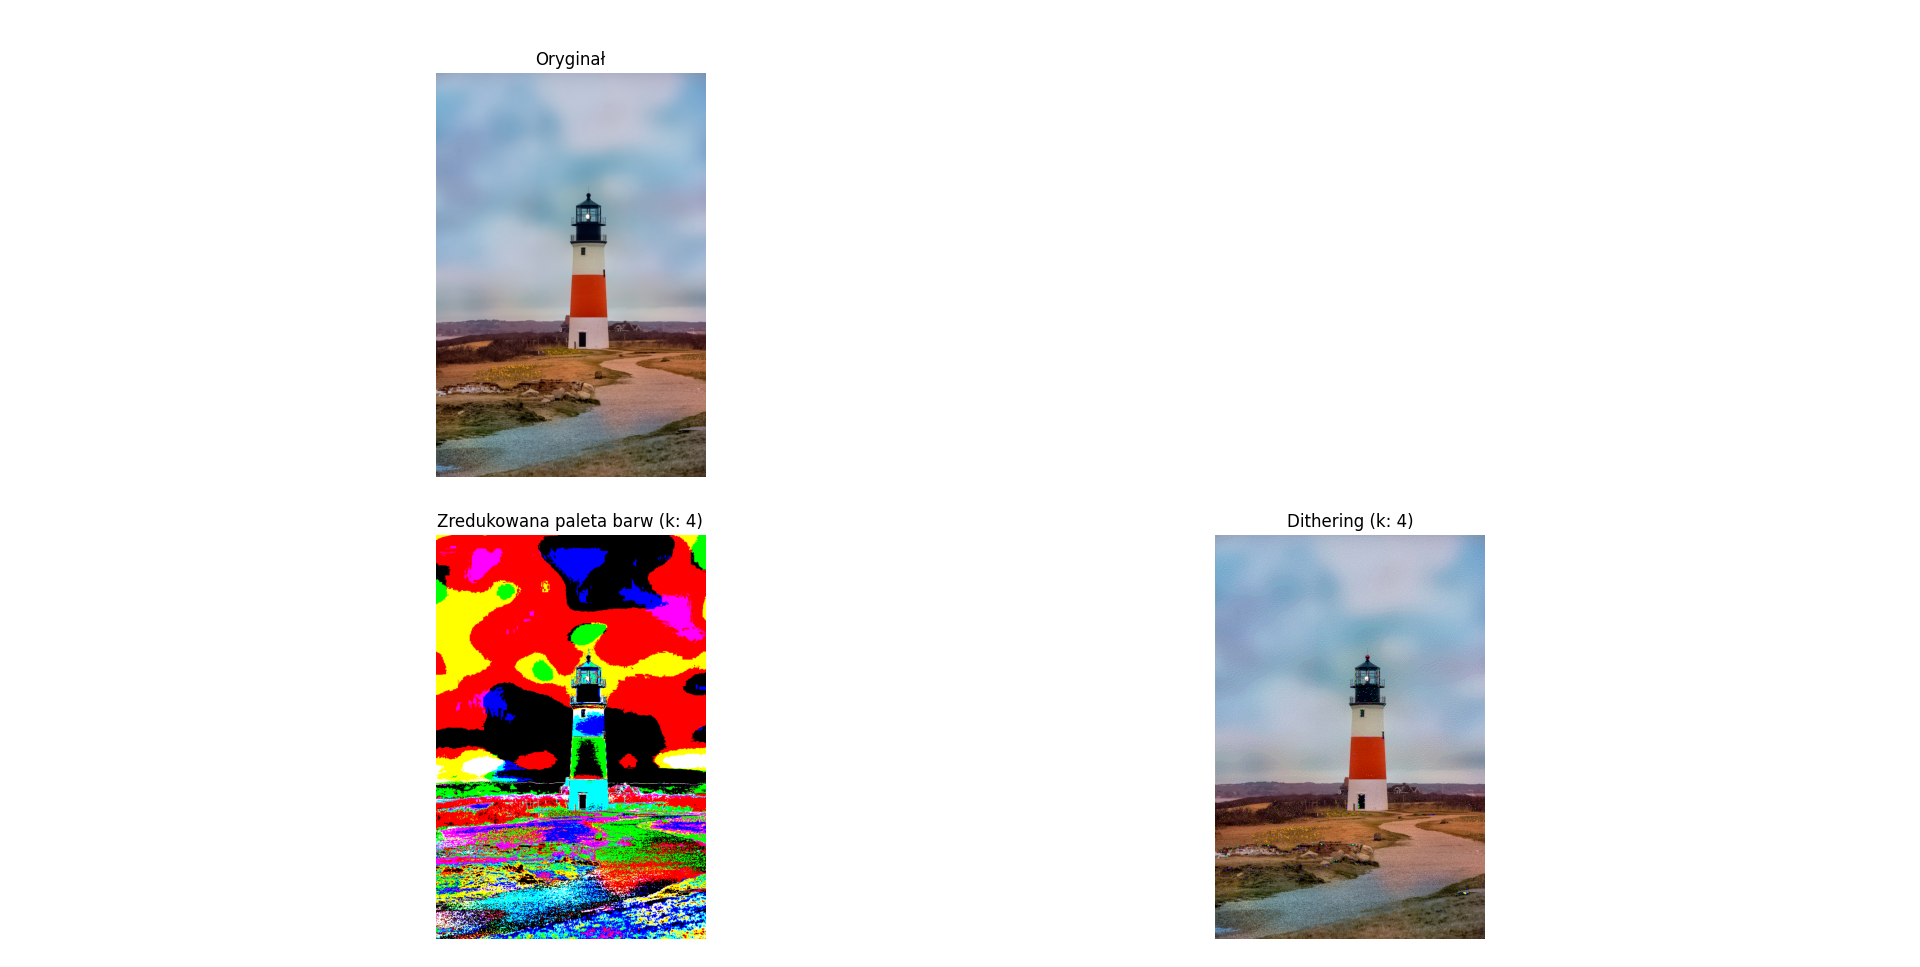
\includegraphics{Img/zad2_4.png}%
    }
    \caption{Zdjęcie przedstawiające obraz oryginalny, obraz po redukcji kolorów i obraz po przetworzeniu (dla k = 4).}
\end{figure}

\begin{figure}[H]
    \centering
    \resizebox{\columnwidth}{!}{%
        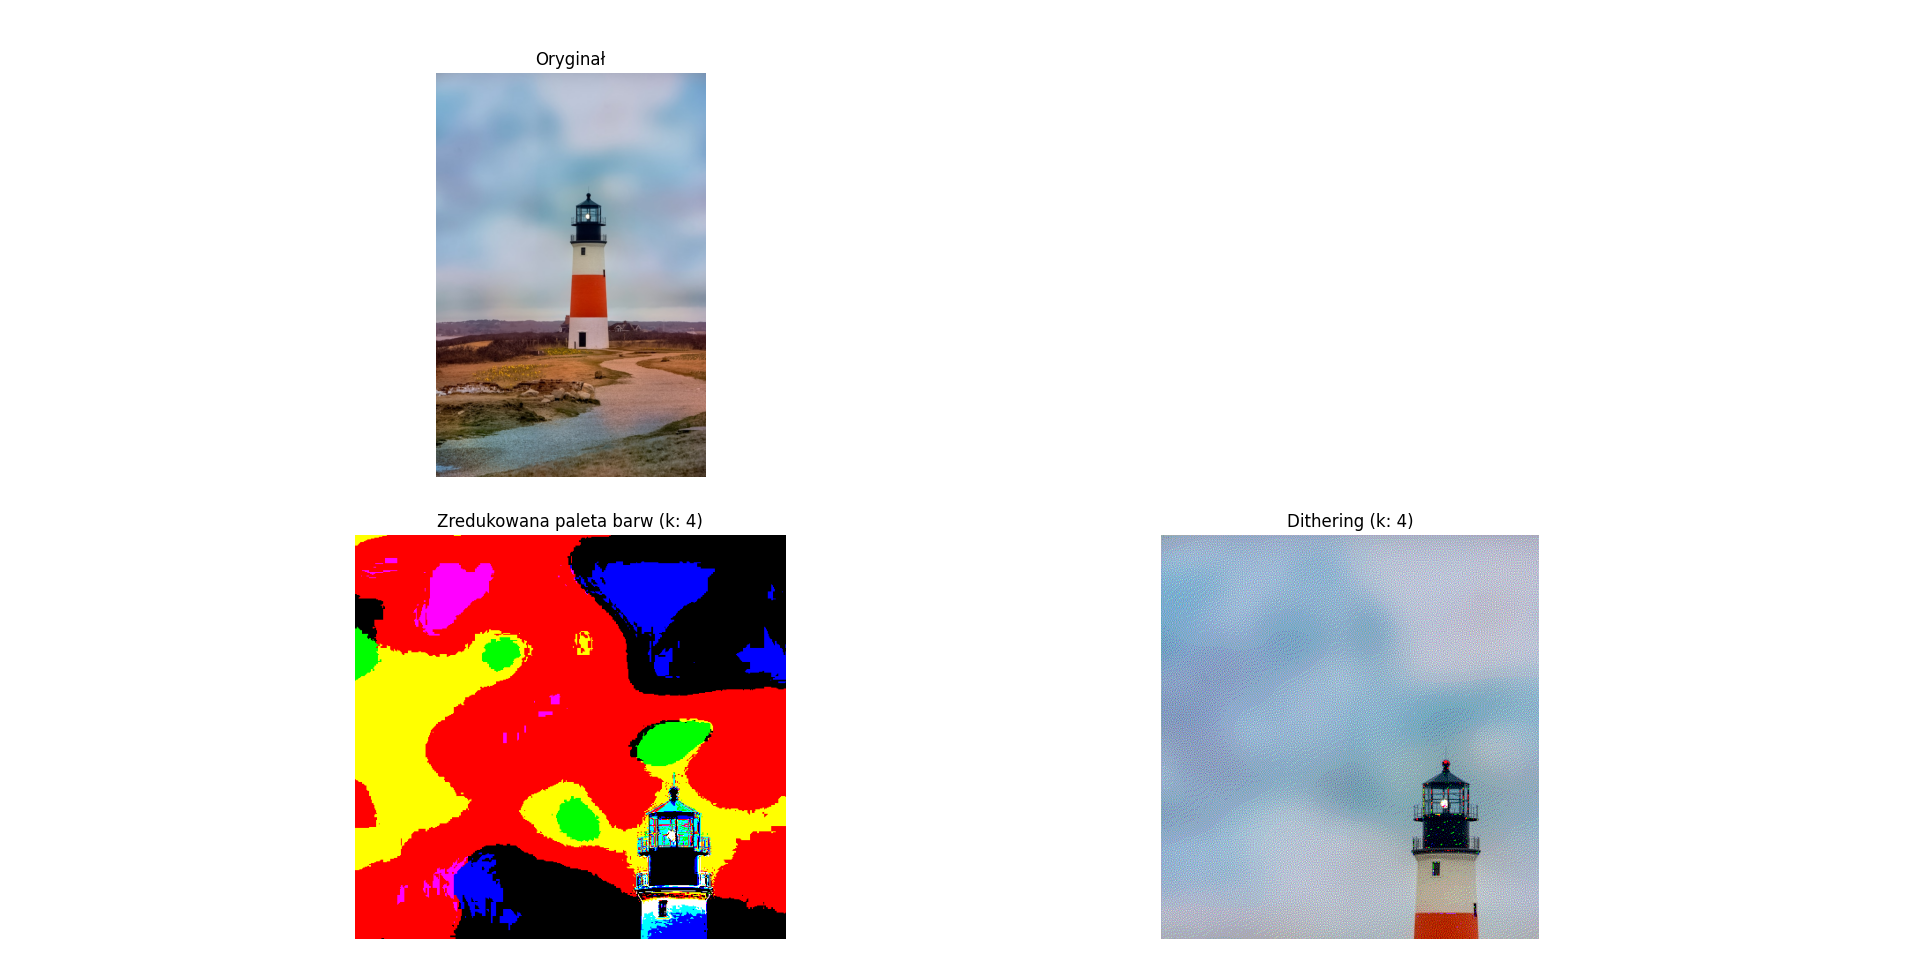
\includegraphics{Img/zad2_5.png}%
    }
    \caption{Zdjęcie przedstawiające obraz oryginalny, przybliżony obraz po redukcji kolorów i przybliżony obraz po przetworzeniu (dla k = 4).}
\end{figure}

\begin{figure}[H]
    \centering
    \resizebox{\columnwidth}{!}{%
        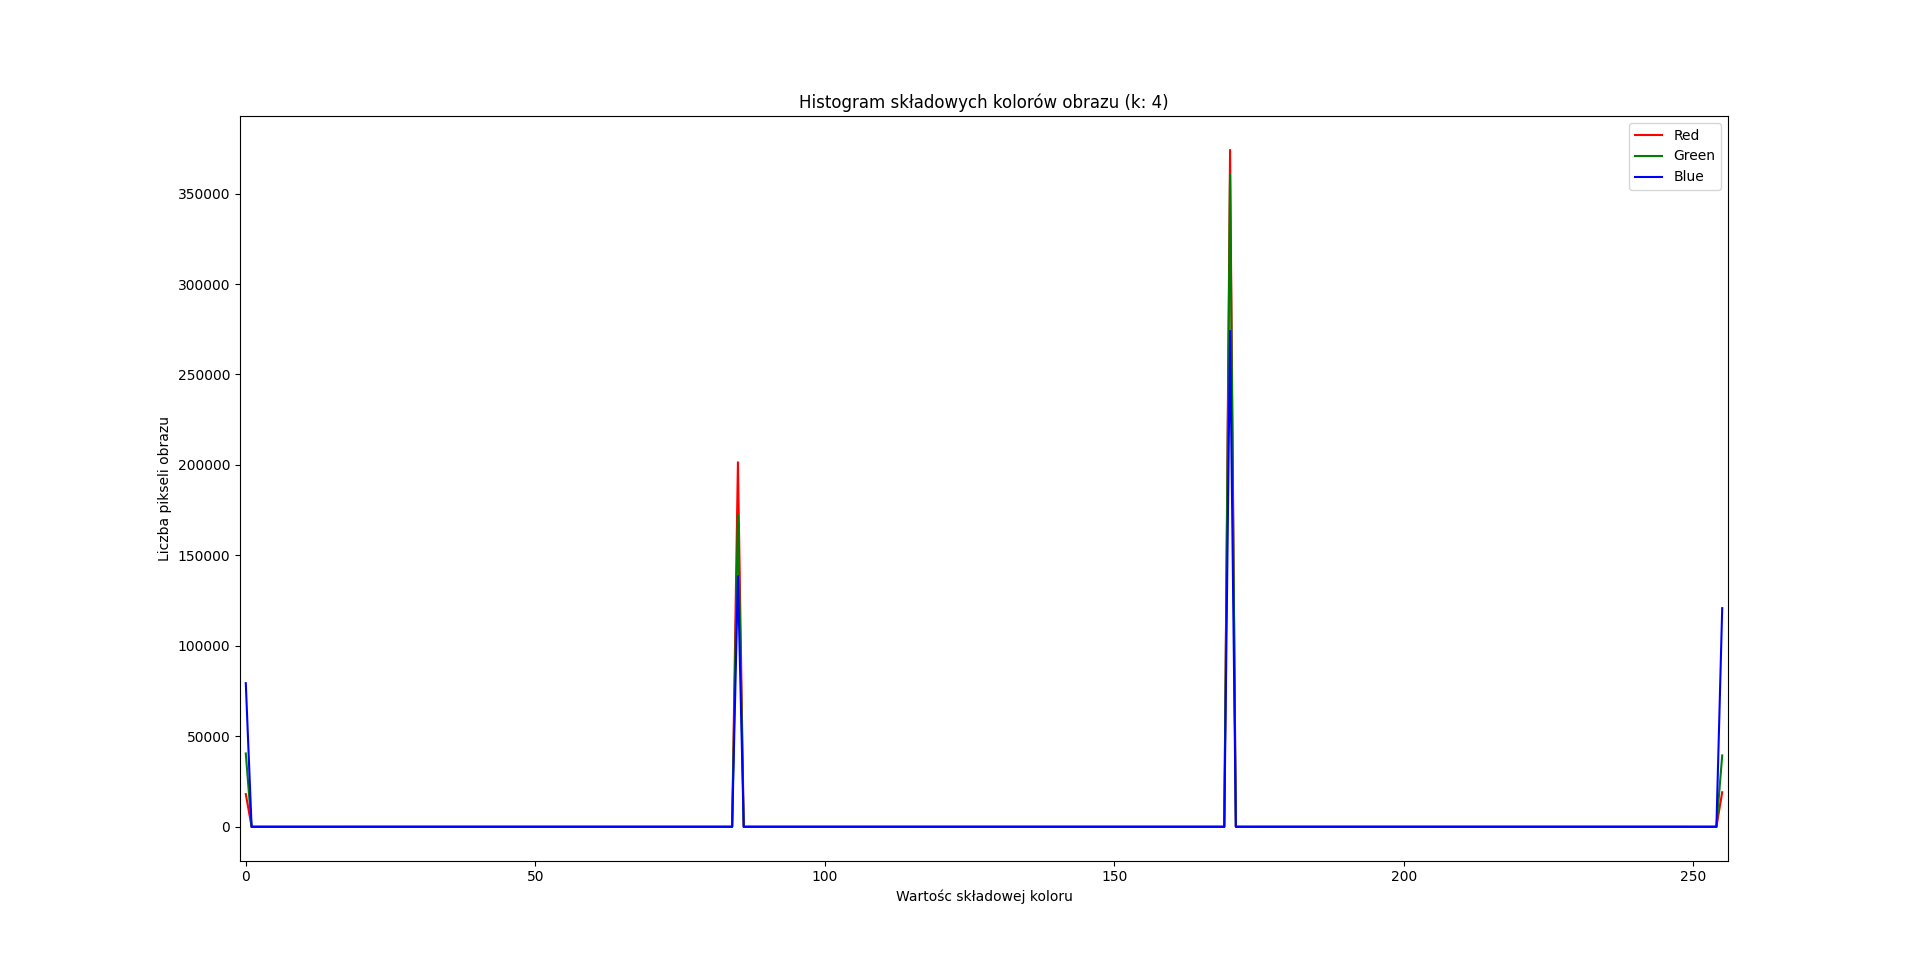
\includegraphics{Img/zad2_6.png}%
    }
    \caption{Zdjęcie przedstawiające histogram składowych kolorów przetworzonego obrazu dla k = 4}
\end{figure}


\section{Zadanie 3}

\subsection{Zadania do wykonania}
Zadanie trzecie polegało na zaimplementowaniu algorytmu Bresenhama do rysowania linii oraz algorytmu do
rysowania trójkątów. Figury miały być jednolite kolorystycznie.

\subsection{Teoria}

\subsubsection*{Algorytm Bresenhama}
Algorytm Bresenhama to wydajna metoda rysowania linii prostych na rastrowym wyświetlaczu komputerowym.
Algorytm działa poprzez iteracyjne wyznaczanie pikseli najbliższych idealnej linii prostej między dwoma
punktami.

Kroki algorytmu Bresenhama:

\begin{enumerate}
    \item Wyznaczenie wielkości pomocniczych:
          \begin{itemize}
              \item Oblicz różnice w pozycjach końcowych punktów linii:
                    \begin{align*}
                         & dx = |x_2 - x_1| \\
                         & dy = |y_2 - y_1|
                    \end{align*}
              \item Określ kierunki kroków
                    \begin{align*}
                         & Xi = 0 \text{ jeżeli } dx = 0 \text{ w innym przypadku } \text{znak}(x_2 - x_1) \\
                         & Yi = 0 \text{ jeżeli } dy = 0 \text{ w innym przypadku } \text{znak}(y_2 - y_1)
                    \end{align*}
          \end{itemize}
    \item Określenie początkowej wartości błędu:
          \begin{itemize}
              \item Jeżeli $dx > dy$ to $d = 2*dy - dx$
              \item Jeżeli $dy > dx$ to $d = 2*dx - dy$
          \end{itemize}
    \item Rysowanie w punkcie początkowym:
          \begin{itemize}
              \item Narysuj piksel w punkcie $(x_0, y_0)$
          \end{itemize}
    \item Powtarzanie w pętli aż do osiągnięcia punktu docelowego:
          \begin{itemize}
              \item Jeżeli $dx > dy$:
                    \begin{itemize}
                        \item $x_0 += Xi$
                        \item $d += 2*dy$
                        \item Jeżeli $d \geq 0$:
                              \begin{itemize}
                                  \item $y_0 += Yi$
                                  \item $d -= 2*dx$
                              \end{itemize}
                    \end{itemize}
              \item Jeżeli $dy > dx$:
                    \begin{itemize}
                        \item $y_0 += Yi$
                        \item $d += 2*dx$
                        \item Jeżeli $d \geq 0$:
                              \begin{itemize}
                                  \item $x_0 += Xi$
                                  \item $d -= 2*dy$
                              \end{itemize}
                    \end{itemize}
          \end{itemize}
\end{enumerate}

gdzie $\text{znak}()$ - funkcja zwracająca znak liczby $(+1 / -1)$

Źródła: \cite{Bresenham}

\subsubsection*{Rysowanie trójkątów}
Trójkąt jest powszechnie używaną figurą w grafice komputerowej. Na jego podstawie buduję się bardziej
skomplikowane kształty, takie jak wielokąty, krzywe czy powierzchnie.

Do rysownia trójkątów można użyć różnych algorytmów, na potrzeby zadania zaimplementowałem algorytm,
którego kroki przedstawiają się następująco:

\begin{enumerate}
    \item Wyznaczenie pomocniczych wartości:
          \begin{itemize}
              \item Wyznaczenie czworokąta otaczającego trójkąt (Trójkąt ma boki: a, b, c. Każdy bok ma składową x i y):
                    \begin{align*}
                         & x_{\text{min}} = \min(a, b, c) \\
                         & y_{\text{min}} = \min(a, b, c) \\
                         & x_{\text{max}} = \max(a, b, c) \\
                         & y_{\text{max}} = \max(a, b, c)
                    \end{align*}
          \end{itemize}
    \item Dla każdego punktu $(p.x, p.y)$ wewnątrz czworokąta:
          \begin{itemize}
              \item Sprawdź, czy punkt znajduje się wewnątrz trójkąta:
                    \begin{align*}
                         & znak_1 = (p.x - a.x)(b.y - a.y)(p.y - a.y)(b.x - a.x) \\
                         & znak_2 = (p.x - b.x)(c.y - b.y)(p.y - b.y)(c.x - b.x) \\
                         & znak_3 = (p.x - c.x)(a.y - c.y)(p.y - c.y)(a.x - c.x)
                    \end{align*}
              \item Jeżeli $znak_1 = znak_2 = znak_3$ to punkt znajduje się wewnątrz trójkąta
          \end{itemize}
\end{enumerate}

Źródła: \cite{barycentryczne1}, \cite{barycentryczne2}

\subsection{Prezentacja wykonanego zadania}
\begin{figure}[H]
    \centering
    \resizebox{\columnwidth}{!}{%
        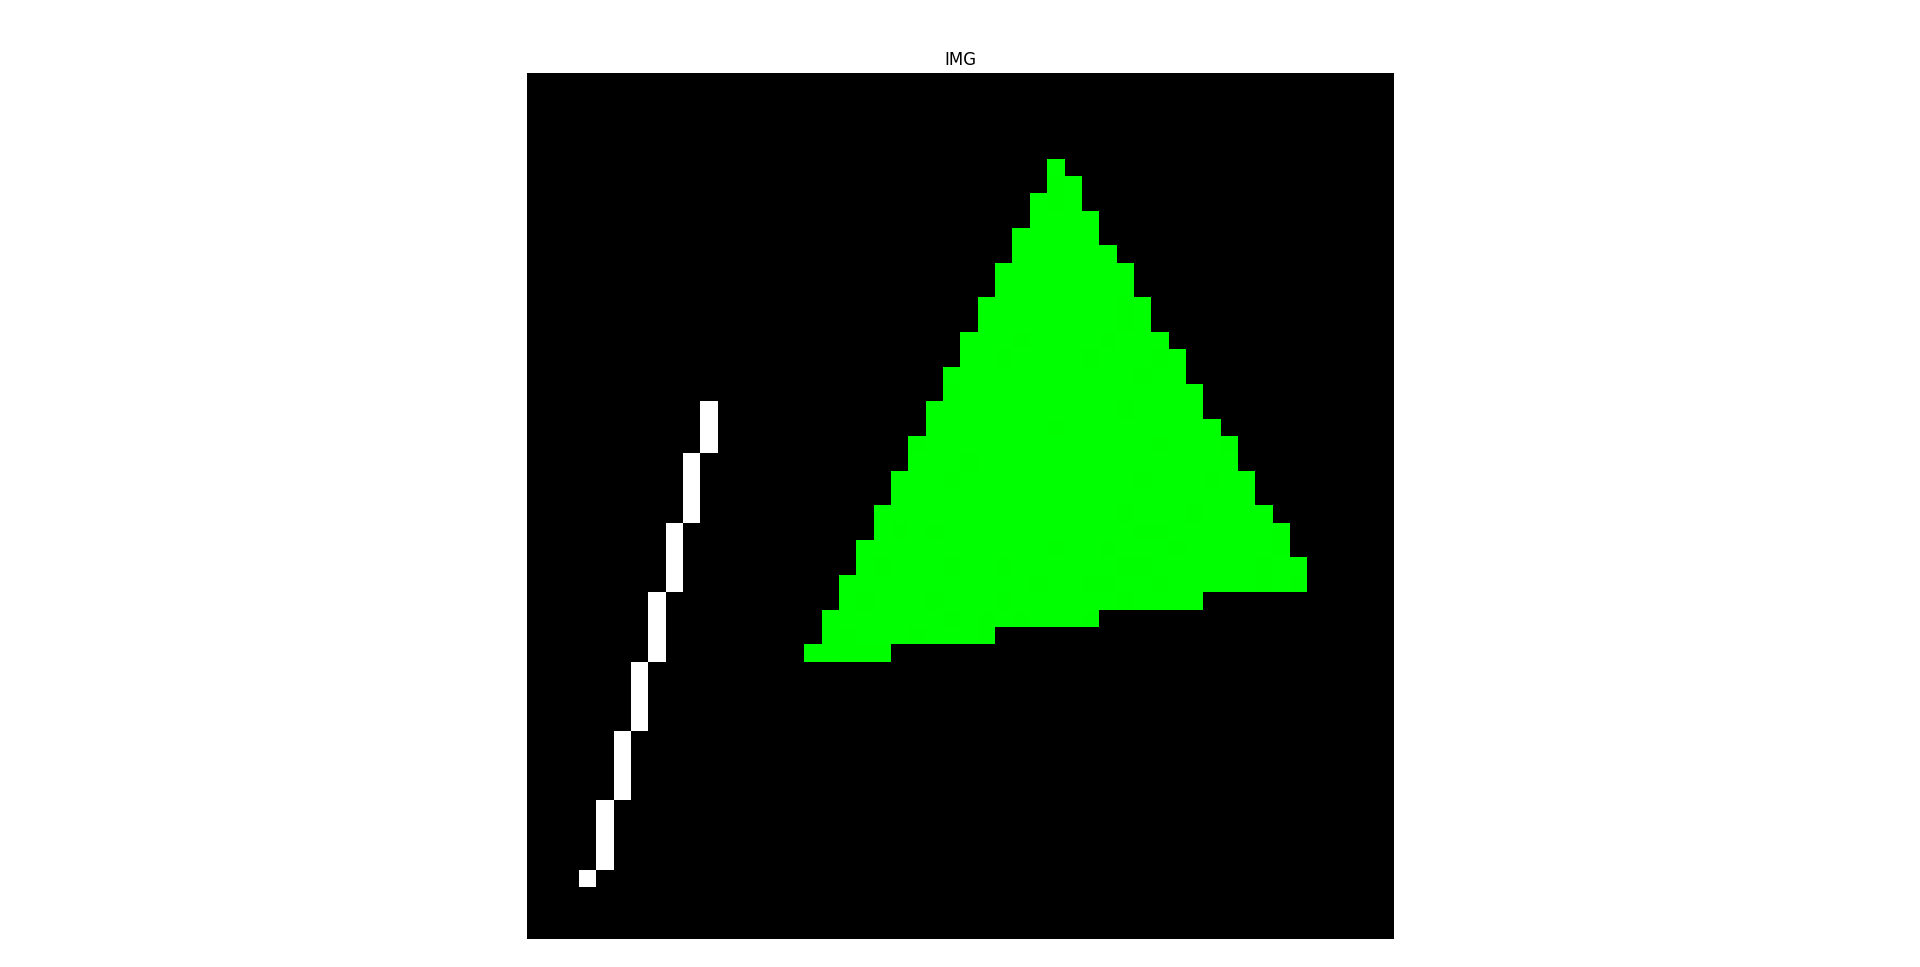
\includegraphics{Img/zad3.png}%
    }
    \caption{Zdjęcie przedstawiające obraz z narysowaną linią i trójkątem.}
\end{figure}

\section{Zadanie 4}

\subsection{Zadania do wykonania}
W tym zadaniu tak samo jak poprzednio mielismy narysować linię i trójkąt, ale tym razem kolory nie miały być
jednolite, a miały byc gradientem.

Dla lini wykorzystałem interpolację liniową koloru w zależności od położenia piksela na linii. Im bliżej
punktu poczatkowego linii tym kolor był bardziej zbliżony do koloru początkowego, a im bliżej punktu końcowego
tym bardziej zbliżony do koloru końcowego.

Dla trójkąta wykorzystałem interpolację barycentryczną. W tym przypadku kolor piksela był obliczany na
podstawie współrzędnych barycentrycznych punktu w trójkącie. Im bliżej jednego z wierzchołków tym kolor był bardziej
zbliżony do koloru tego wierzchołka.

\subsection{Prezentacja wykonanego zadania}
\begin{figure}[H]
    \centering
    \resizebox{\columnwidth}{!}{%
        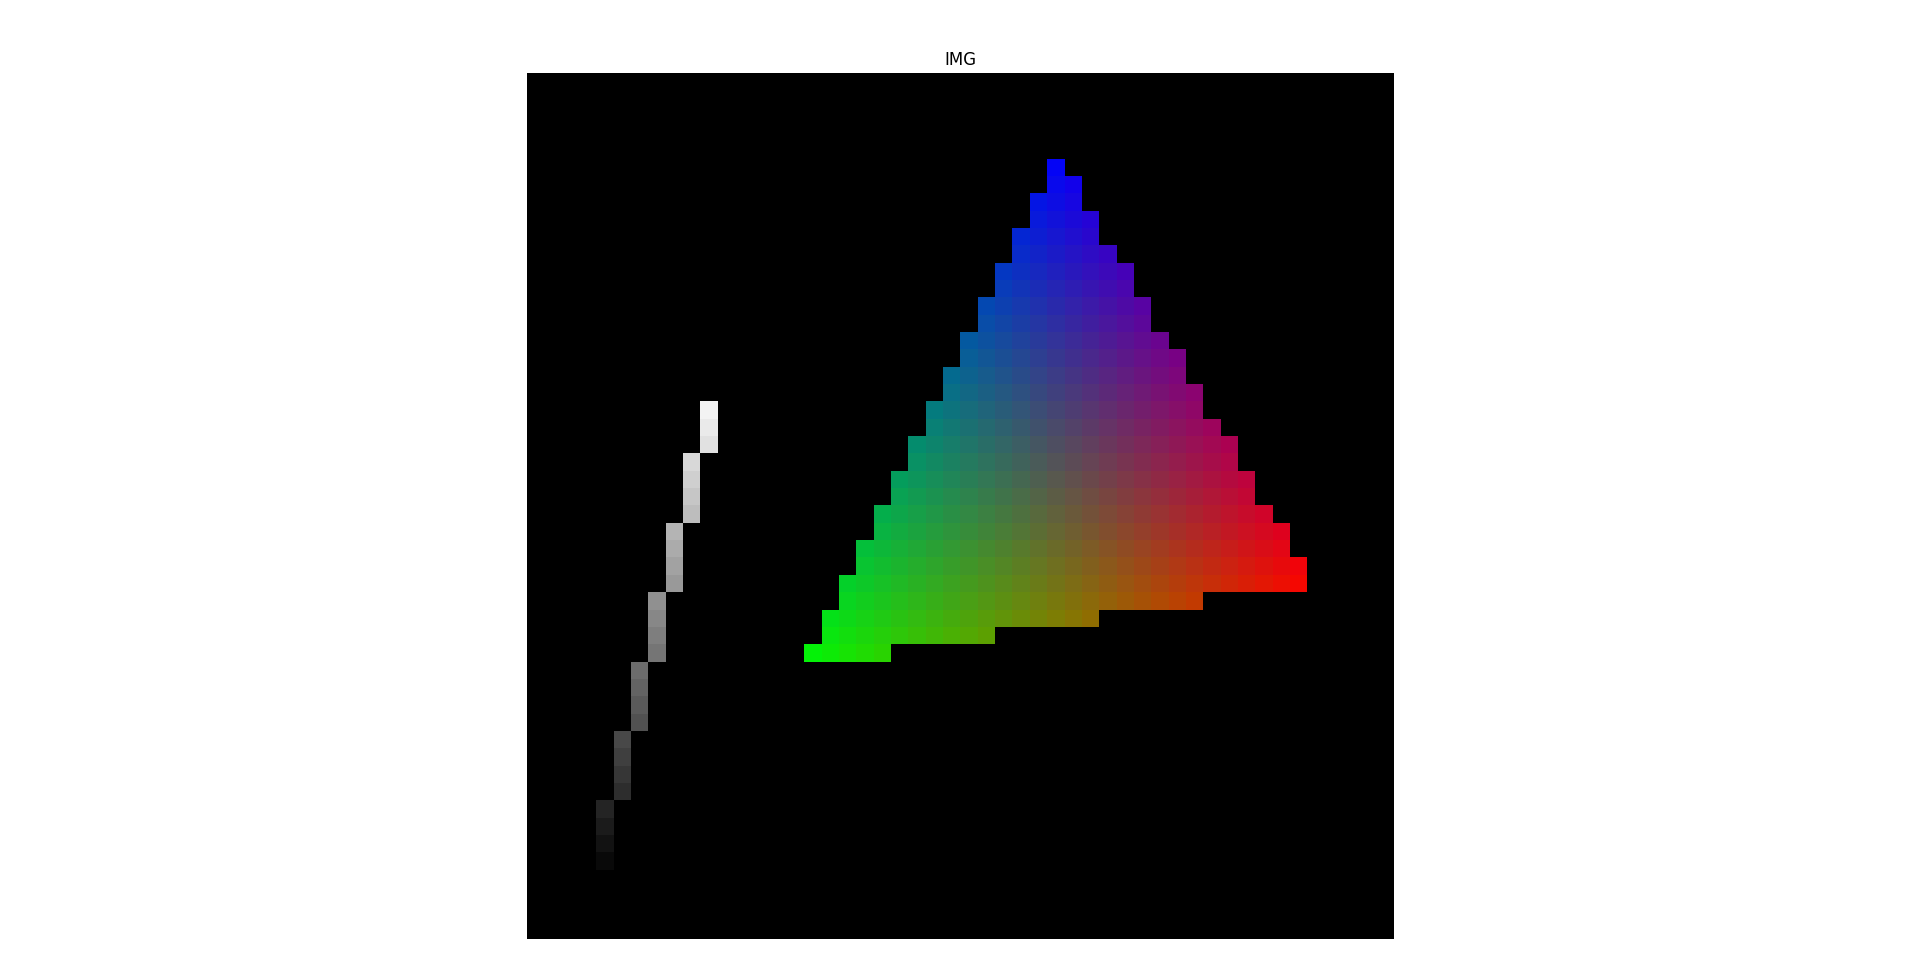
\includegraphics{Img/zad4.png}%
    }
    \caption{Zdjęcie przedstawiające obraz z narysowaną linią i trójkątem z gradientem kolorów.}
\end{figure}

\section{Zadanie 5}

\subsection{Zadania do wykonania}
W ramach zadania piątego mieliśmy zaimplementować wygładzanie krawędzi w generowanym obrazie.
W tym celu wykorzystaliśmy algorytm SSAA (Super Sampling Anti Aliasing).

Algorytm SSAA polega na generowaniu obrazu o większej rozdzielczości niż docelowa, a następnie
zmniejszeniu go do docelowej rozdzielczości. W ten sposób uzyskujemy wygładzenie krawędzi.

Zaimplementowany algorytm najpierw rysuję obraz dwukrotnie większy niż docelowy,
a następnie z każdych czterech pikseli oblicza średni kolor i rysuje go na obrazie docelowym.

\subsection{Prezentacja wykonanego zadania}
\begin{figure}[H]
    \centering
    \resizebox{\columnwidth}{!}{%
        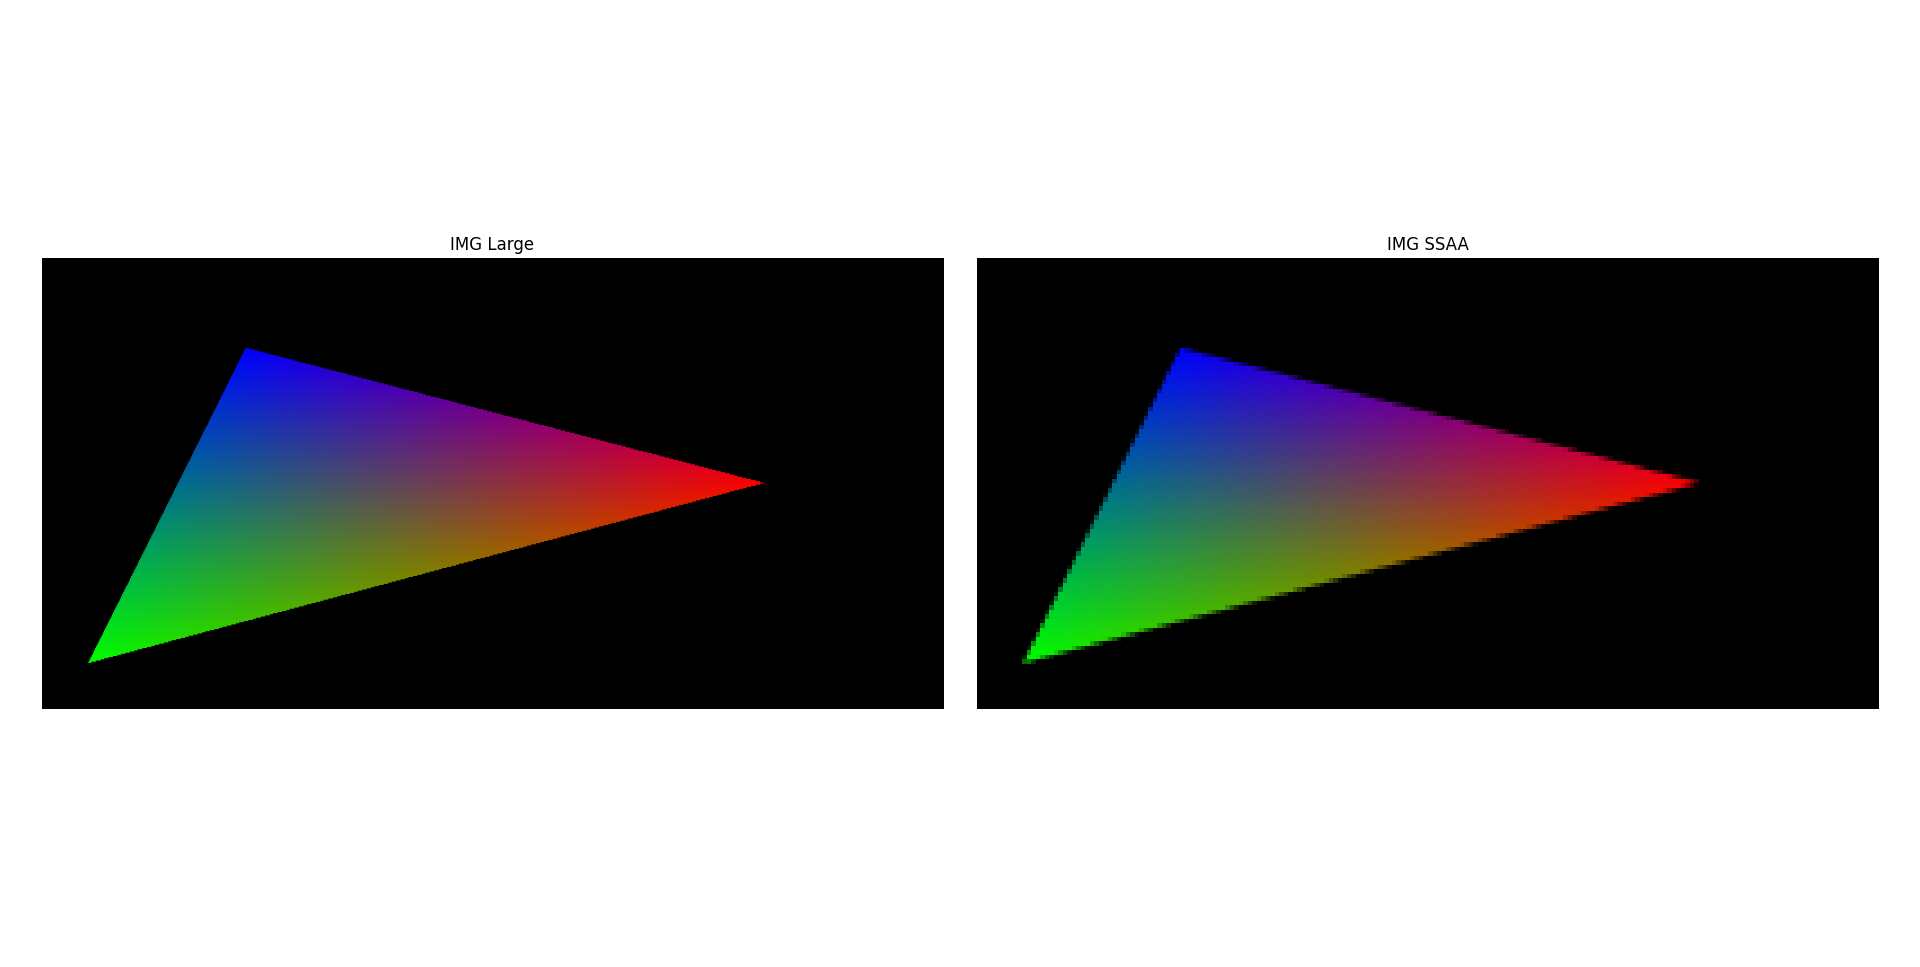
\includegraphics{Img/zad5.png}%
    }
    \caption{Zdjęcie przedstawiające obraz z wygładzonymi krawędziami.}
\end{figure}

\begin{figure}[H]
    \centering
    \resizebox{\columnwidth}{!}{%
        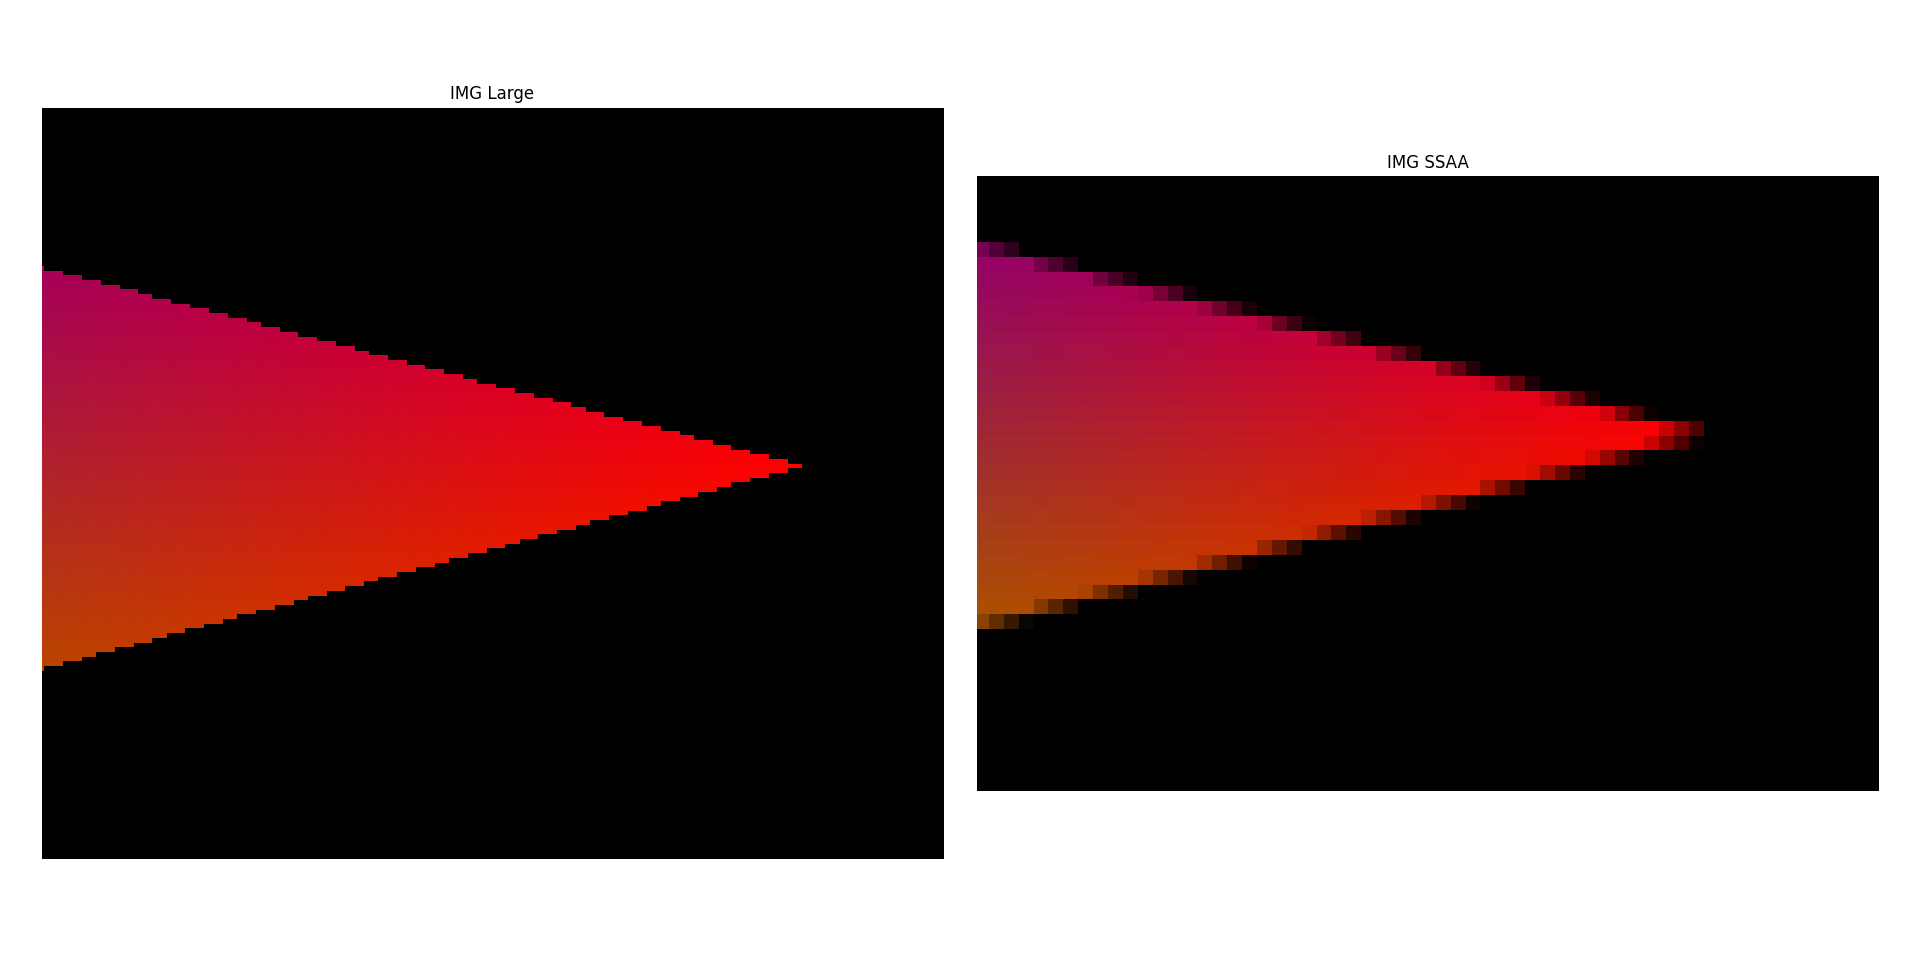
\includegraphics{Img/zad5_2.png}%
    }
    \caption{Zdjęcie przedstawiające obraz z wygładzonymi krawędziami (przybliżenie).}
\end{figure}


\bibliographystyle{plainnat}
\bibliography{TexBase/Bibliography}

\end{document}